% -*- root: ../AlgebraConmutativa.tex -*-
\chapter{Anillos de coordenadas y morfismos entre variedades}

Una vez que ya hemos presentado los objetos que querremos estudiar (las variedades algebraicas), vamos a describir los tipos de funciones que podremos definir sobre las variedades algebraicas afines.

\begin{defn}[Función\IS regular] Sea $X ⊂ \afesp$ una variedad algebraica afín. Diremos que $\appl{f}{X}{\K}$ es regular en $X$ si existe un polinomio $F(x_1, \dotsc, x_n) ∈ \K[x_1, \dotsc, x_n]$ tal que $∀(a_1, \dotsc, a_n) ∈ X$, se tiene que $f(a_1, \dotsc, a_n) = F(a_1, \dotsc, a_n)$.

Es decir, $f$ será regular si y sólo si hay un polinomio $F(x_1, \dotsc, x_n) ∈ \K[x_1, \dotsc, x_n]$ tal que $\restr{F}{X} = f$.
\end{defn}

\begin{example}
\begin{itemize}
\item En $\afesp[ℝ][2]$, podemos fijarnos en la recta $X = \set{y = 0}$ y en la función $f(a,b) = a + \sin b$. Sobre $X$, $f$ es regular ya que podemos tener el polinomio $F(x,y) = x$ que es igual a $f$ en todos los puntos de $X$. Ahora bien, $f$ no sería regular sobre todo $\afesp[ℝ][2]$ porque el seno no va a poder expresarse como un polinomio (finito).
\item Dado $\afesp[\K][2] ⊃ Y = \set{y^2 - x = 0}$, y $g(a,b) = a$, que es regular sobre $Y$. Si tomásemos $g(a,b) = a + (a^3 + 3 \sin b) (b^2 - a)$, sigue siendo regular porque la parte conflictiva desaparece.
\end{itemize}
\end{example}

Podemos ver que siempre tenemos al menos una función regular en variedades $X$: al menos tenemos la función $0$ que siempre es regular. Además, la suma de dos funciones regulares seguirá siendo regular, el producto también, y tenemos un neutro para la suma (la función $0$) y el producto (la función $1$). Así, podremos estudiar el anillo conmutativo y con unidad de funciones regulares sobre $X$, que describiremos como \( \label{eq:AnilloFuncRegulares} Γ(X, \K) ≝ \set{\appl{f}{X}{\K} \tq f\text{ es regular}} \)

Para poder hacer cuentas, querremos identificar y saber quién es ese anillo. Para ello, vemos que hay una relación entre los polinomios de $\K[x_1, \dotsc, x_n]$ y $Γ(x,\K)$:
\begin{align*}
\appl{ψ}{\K[x_1, \dotsc, x_n]&}{Γ(X, \K)} \\
p(x_1, \dotsc, x_n) &\longmapsto \appl{f_p}{X}{\K} \\
&\phantom{\longmapsto f_p:}\quad \va \longmapsto p(\va)
\end{align*} con $\va ∈ X$.

Esta función ψ es un homomorfismo de anillos trivialmente. Además, es sobreyectivo. Para ello, tomamos $f ∈ Γ(X, \K)$, está claro que existe un polinomio $p ∈ \K[x_1, \dotsc, x_n]$ tal que $ψ(p) = f$ , por la propia definición de función regular.

Una vez que sabemos que es sobreyectivo, podemos aplicar el \nref{thm:IsomorfiaAnillos1} y sabemos que \[ \quot{\K[x_1, \dotsc, x_n]}{\ker ψ} \simeq Γ(X,\K) \]

Querríamos saber entonces quién es $\ker ψ$, que será el conjunto siguiente: \[ \ker ψ = \set{ p(x_1, \dotsc, x_n) ∈ \K[x_1, \dotsc, x_n] \tq \restr{ψ(p(x_1, \dotsc, x_n))}{X} = 0} \]

En otras palabras, $\ker ψ = \I(X)$. Una vez hecho esto ya podremos definir bien $Γ$ y darle la notación definitiva.

\begin{defn}[Anillo\IS de coordenadas de $X$] Sea $X ⊂ \afesp$. Entonces, se define el anillo de funciones regulares en $X$ o anillo de coordenadas de $X$ como \[ \K[X] ≝ \quot{\K[x_1, \dotsc, x_n]}{\I(X)} \simeq Γ(X, \K)\]
\end{defn}

Este anillo es siempre reducido porque $\I(X)$ es radical.

A través de este anillo podremos estudiar la variedad. Por ejemplo, podremos saber su dimensión, si es irreducible ($\K[X]$ debería de ser dominio de integridad) o si tiene picos.

De momento, lo que empezaremos estudiando serán los morfismos entre las variedades algebraicas a través de este anillo de coordenadas.

\section{Morfismos entre variedades algebraicas afines}

\begin{defn}[Morfismo\IS entre variedades algebraicas afines] Sean $X ⊆ \afesp$ y $Y ⊆ \afesp[\K][m]$ dos variedades algebraicas afines definidas sobre el mismo cuerpo $\K$. Un morfismo $\appl{φ}{X}{Y}$ es una función cuyas coordenadas son funciones regulares en $X$, de tal forma que \[ φ(a_1, \dotsc, a_n) = \left(f_1(a_1, \dotsc, a_n), \dotsc, f_m(a_1, \dotsc, a_n)\right)\] con $f_i$, $i = 1, \dotsc, m$ regulares en $X$.
\end{defn}

\begin{example}
La aplicación \begin{align*}
\appl{φ}{\afesp[\K][1]&}{\afesp[\K][2]} \\
(a) &\longmapsto (a,0)
\end{align*} es un morfismo entre variedades. En general, podríamos también considerar $(a) \longmapsto (p_1(a), p_2(a))$ con $p_i ∈ \K[\afesp[\K][1]] = \K[x]$ (esta última igualdad sólo si \K es infinito), que es lo que esperábamos que pasase.

Igualmente, una proyección \begin{align*}
\afesp[\K][3] &\longmapsto \afesp[\K][2] \\
(a_1, a_2, a_3) &\longmapsto (a_1, a_2)
\end{align*} también será un morfismo.
\end{example}

\notacion: Llamamos $\cls{x_i}$ a la i-ésima función coordenada, que es una función regular y que hace lo siguiente:

\begin{align*}
	\cls{x_i}: X & \rightarrow Y \\
	(a_1,...,a_n) & \rightarrow a_i
\end{align*}

Una cosa que esperaríamos es que los morfismos nos lleven funciones regulares en funciones regulares definidas sobre ambos anillos de coordenadas. Y como a veces el mundo matemático es justo, es precisamente lo que va a ocurrir.

\begin{prop} \label{prop:induce}
Sean $X ⊆ \afesp$ y $Y ⊆ \afesp[\K][m]$ dos variedades algebraicas afines definidas sobre el mismo cuerpo $\K$, y sea φ un morfismo $X \rightarrow Y$. Entonces φ induce un homomorfismo de anillos $\appl{f_φ}{\K[Y]}{\K[X]}$.
\end{prop}


\notacion A veces llamaremos a $f_{\varphi}=\varphi^*$.

\notacion Este homomorfismo de anillos de coordenadas lo que hace es enviar una función coordenada $\cls{y_i}$ a la cual se le asocia la función regular $f_i$. Por tanto, si me fijo en una función regular cualquiera en $\cls{G(y_1,...,y_n)} \in \K[Y]$ (que no es un polinomio sino una clase de polinomios y por ello le ponemos la barra) esta va a parar en $\cls{G(f_1,...,f_m)}$:

\begin{align*}
	\varphi^*: \K[Y] & \rightarrow \K[X] \\
	\cls{y_i} & \rightarrow f_i\\
	\cls{G(y_1,...,y_n)} & \rightarrow \cls{G(f_1,...,f_m)}
\end{align*}

\begin{example}
	$G(y_1,y_2)= y_1^2+2y_2 \rightarrow f_1^2+2f_2$
\end{example}

\begin{proof} Dada una aplicación $g ∈ \K[Y]$, entonces $g ○ φ$ es una aplicación $\appl{g ○ φ}{X}{\K}$. Hay que demostrar que es un homomorfismo de anillos.

Como tratar de construir un homomorfismo de cocientes a cocientes es arriesgado, lo que haremos será definir un homomorfismo de $\K[y_1, \dotsc, y_m]$ a $\K[X]$ y después ver que factoriza por el cociente. El homomorfismo lo definiremos de la siguiente forma: dejaremos fijos los $r ∈ \K$, y cada variable $y_i$ la consideraremos como función regular en $\K[Y]$. Decíamos antes que la aplicación que definiríamos $X \longmapsto \K$ sería la composición con φ, así que lo que hacemos es ver qué ocurre cuando $g = \cls{y_i}$: \[
\begin{matrix}
X &\xrightarrow{φ}& Y &\xrightarrow{y_i}& \K \\
(a_1, \dotsc, a_n) &\longrightarrow & \left(f_1(a_1, \dotsc, a_n), \dotsc, f_m(a_1, \dotsc, a_n)\right) &\longrightarrow & f_i(a_1, \dotsc, a_n)
\end{matrix}\]

Así, el homomorfismo que definiremos será
\begin{align*}
f_{\varphi}: \K[y_1, \dotsc, y_m] &\longmapsto \K[X] = \quot{\K[x_1, \dotsc, x_n]}{\I(X)} \\
r ∈ \K &\longmapsto r ∈ \K \\
y_i &\longmapsto \cls{f_i(x_1,\dotsc, x_n)}
\end{align*}


%Clase 11/04/2016


Esta $\I(Y) \subset \ker(f_{\varphi})$?? Sabemos que $\I(Y) \subset \K[y_1,...,y_m]$. Sea $G \in \I(Y) \implies \forall (b_1,...,b_m) \in Y \implies G(b_1,...,b_m)=0$. Queremos ver que $f_{\varphi}(G)=0$.

Entonces $f_{\varphi}(G)=G(f_1,...,f_m) \in \K[X]=\quot{\K[x_1,...,x_n]}{\I(X)}$ ¿Cuándo $G(f_1,...,f_m)=0$ en $\K[X]$?

$G(f_1,...,f_n)=0$ en $\K[X] \Leftrightarrow \forall (a_1,...,a_n) \in X$, $G(f_1,...,f_n)(a_1,...,a_n)=0 \Leftrightarrow G(f_1(a_1,...,a_n),...,f_m(a_1,...,a_n))=0 \; \forall(a_1,..,a_n) \in X$.

Sabiendo que $G \in \I(Y)$ podemos asegurar que $G(f_1(a_1,...,a_n),...,f_m(a_1,...,a_n))=0$ $\forall (a_1,...,a_n) \in X$??

Pues bien, tenemos
\begin{align*}
	X & \rightarrow Y \\
	(a_1,...,a_n) & \rightarrow (f_1(a_1,...,a_n),...,f_m(a_1,...,a_n))
\end{align*}
Entonces $(f_1(a_1,...,a_n),...,f_m(a_1,...,a_n)) \in Y \; \forall (a_1,...,a_n) \in X \implies G\underbrace{(f_1(a_1,...,a_n),...,f_m(a_1,...,a_n))}_{\in Y}=0$ ya que $G \in \I(Y) \implies $
\begin{align*}
	\K[y_1,...,y_m] & \stackrel{f_{\varphi}}{\rightarrow} \K[X] \\
	y_i & \rightarrow f_i
\end{align*}

Factoriza por $\quot{\K[y_1,..,y_n]}{\I(Y)}$ y por tanto induce un homomorfismo de anillos $\cls{f_{\varphi}}: \K[Y] \rightarrow K[X]$
\end{proof}

\nota En algunos ejemplos al considerar espacios afines $\Akn$ y mirar a sus anillos de coordenadas tendremos que: $\K[\Akn]=\quot{\K[x_1,...,x_n]}{\I(\Akn)}=\K[x_1,...,x_n]$ si $|K|=\infty$.

\begin{example}
	Cogemos $X=\A_K^2$ e $Y=\A_K^3$:
	\begin{align*}
		\A_K^2 & \rightarrow \A_K^3 \\
		(a_1,a_2) & \rightarrow (a_1,a_2,0)
	\end{align*}

	Tendríamos que: $$\K[X]=\quot{\K[x_1,x_2]}{\I(X)}=\quot{\K[x_1,x_2]}{\{0\}} = \K[x_1,x_2]$$

	$$ K[Y]=\quot{\K[y_1,y_2,y_3]}{\I(X)}=\quot{\K[y_1,y_2,y_3]}{\{0\}} = \K[y_1,y_2,y_3] $$

	Y según el teorema tenemos el siguiente homomorfismo en anillos de coordenadas:
	\begin{align*}
		K[y_1,y_2,y_3] & \rightarrow \K[x_1,x_2] \\
		y_1 & \rightarrow x_1 \\
		y_2 & \rightarrow x_2 \\
		y_3 & \rightarrow 0 \\
	\end{align*}
\end{example}


	\begin{example}
		\begin{align*}
			\A_K^3 & \rightarrow \A_K^2 \\
			(a_1,a_2,a_3) & \rightarrow (a_1,a_2)
		\end{align*}

		Y según el teorema tenemos el siguiente homomorfismo en anillos de coordenadas:
		\begin{align*}
			K[y_1,y_2] & \rightarrow \K[x_1,x_2,x_3] \\
			y_1 & \rightarrow x_1 \\
			y_2 & \rightarrow x_2 \\
		\end{align*}
	\end{example}

	\begin{example}
		Cogemos la hipérbola $H=\{x_1x_2-1=0\}$, cogemos un punto y lo dejamos caer.
		\begin{align*}
			H=\{x_1x_2-1=0\} & \rightarrow \A_K^1 \\
			(a_1,a_2) & \rightarrow a_1
		\end{align*}

		Y según el teorema tenemos el siguiente homomorfismo en anillos de coordenadas:
		\begin{align*}
			K[y_1] & \rightarrow \quot{\K[x_1,x_2]}{\gen{x_1x_2-1}} \simeq \K[x_1]_{\{x_1\}} \\
			y_1 & \rightarrow x_1 \\
		\end{align*}

		Lo de que $\quot{\K[x_1,x_2]}{\gen{x_1x_2-1}} \simeq \K[x_1]_{\{x_1\}}$ parece un poco by the face, pero vamos, es básicamente que al poner $x_1x_2-1$ lo que estamos haciendo realmente es añadir a $\K[x_1]$ los elementos inversos de $x_1$, que es precisamente lo que significa localizar en $x_1$.

		El homomorfismo que hemos definido además es una inclusión, es decir $K[y_1] \subset \quot{\K[x_1,x_2]}{\gen{x_1x_2-1}}$. Si no fuera por el cociente lo veríamos clarísisisisisimo, el cociente jode un poco, pero podemos decir que es una inclusión porque si no lo fuese habría algun polinomio no nulo en $Y$ cuya imagen caería dentro del ideal $\gen{x_1x_2-1}$. Pero un polinonmio no nulo en $Y$ es un polinomio no nulo en $x_1$ y estaríamos diciendo que ese polinomio pertenecería a $\gen{x_1x_2-1}$, lo cual es imposible porque no tendríamos $x_2$.  Otra forma de verlo más es sencillo es con lo de que $\quot{\K[x_1,x_2]}{\gen{x_1x_2-1}} \simeq \K[x_1]_{\{x_1\}}$, aquí se ve mas claro, pues estoy añadiendo a $\K[x_1]$ más elementos.

		Es inyectiva pero no es sobreyectiva %(PERO POR POCOO! ya que el único punto al que no llego es al 0).
	\end{example}

	\begin{example}
		Cogemos la parábola $X=\{x_2^2-x_1=0\}$, cogemos un punto y lo dejamos caer.
		\begin{align*}
			X=\{x_2^2-x_1=0\} & \rightarrow \A_K^1 \\
			(a_1,a_2) & \rightarrow a_1
		\end{align*}

		Y según el teorema tenemos el siguiente homomorfismo en anillos de coordenadas:
		\begin{align*}
			K[y_1] & \rightarrow \quot{\K[x_1,x_2]}{\gen{x_2^2-x_1}} \\
			y_1 & \rightarrow x_1
		\end{align*}

		El homomorfismo es una inclusión como antes. $x_2$ es entero sobre $\K[x_1]$. Es decir $\cls{x_2}$ es raíz del $p(t)=t^2-x_1$, $p(t)\in \K[x_1][t] \implies \quot{\K[x_1,x_2]}{\gen{x_2^2-x_1}}$ es una extensión finita (y por tanto entera) de $\K[y_1]$ vía f.
	\end{example}

	\begin{prop}
		Sean $X \subseteq \Akn$ e $Y \subseteq \Akn$ v.a.a.. Todo homomorfismo de anillos $f: \K[Y] \rightarrow \K[X]$ induce un morfismo $\varphi_g: X \rightarrow Y$ de K-álgebras (los elementos de $\K$ se quedan fijos).
	\end{prop}

	\begin{proof}
		Tengo lo siguiente:

		\begin{tikzcd}
			\quot{\K[y_1,...,y_m]}{\I(Y)} \arrow[rightarrow]{rr}{f}
			\arrow[leftarrow]{dr}{}
			& & \begin{matrix}
				\quot{\K[x_1,...,x_n]}{\I(X)} \\ f_1
			\end{matrix}  \arrow[leftarrow]{dl}\\
			& \begin{matrix}
				\K[y_1,...,y_m] \\y_1
			\end{matrix}&
		\end{tikzcd}

		Queremos inducir un homomorfismo $\varphi_g: X \rightarrow Y$.

		Si escogemos m funciones regulares tendremos:


		\begin{align*}
			X & \rightarrow \A_K^m \\
			(a_1,...,a_n) & \rightarrow (f_1(a_1,...,a_n),...,f_m(a_1,...,a_n))
		\end{align*}

		Entonces queremos probar que $(f_1(a_1,...,a_n),...,f_m(a_1,...,a_n)) \in Y$. Es decir, si $(a_1,...,a_n) \in X \implies (f_1(a_1,...,a_n),...,f_m(a_1,...,a_n)) \in Y$???

		Entonces $(f_1(a_1,...,a_n),...,f_m(a_1,...,a_n)) \in Y \Leftrightarrow \forall G \in \I(Y)$, $G(f_1(a_1,...,a_n),...,f_m(a_1,...,a_n))=0$.

		Sea $G\in \I(Y)$ queremos ver si $G(f_1(a_1,...,a_n),...,f_m(a_1,...,a_n))=0$.

		$$G(f_1(a_1,...,a_n),...,f_m(a_1,...,a_n))=G(f_1,...,fm)(a_1,...,a_m)= \underbrace{\hat{g}(G)}_{=0 \text{ porque } \I(Y) \subset \ker(g)}(a_1,...,a_m)$$

		$\hat{g}(G) \in \ker \hat{g} \implies \hat{g}(G) \equiv 0$ en $X$ $\implies \forall(a_1,...,a_n) \in X$, $\hat{g}(G)(a_1,...,a_n)=0$
	\end{proof}

%clase 13/04/2016

\begin{lemma}
	Sean $X,Y,Z$ v.a.a sobre el mismo cuerpo $\K$ y sean $\varphi:X \rightarrow Y$ e $\psi: Y \rightarrow Z$ morfismos, entonces:
	\begin{enumerate}
		\item $\psi \circ \varphi: X \rightarrow Z$ es un morfismo:
		\item $(\psi \circ \varphi)^*: \K[Z] \rightarrow \K[X]$ y $(\psi \circ \varphi)^*=\psi^* \circ \varphi^*$
		\item

		\begin{align*}
		Id_X: X & \rightarrow X \\
		(a_1,...,a_n) & \rightarrow (a_1,...,a_n)
		\end{align*}

		con $f_i=\cls{x_i}\in  \K[X]=\quot{\K[x_1,...,x_n]}{\I(X)} \implies Id_X^*: \K[X] \rightarrow \K[X]$ es el homomorfismo identidad en $\K[X]:Id_{\K[X]}$
	\end{enumerate}
\end{lemma}

\nota Podemos aplicar lo mismo si en vez de $X,Y,Z$ v.a.a tenemos $\K[X], \K[Y], \K[Z]$ y $\varphi^*:\K[X] \rightarrow \K[Y]$ e $\psi^*: \K[Y] \rightarrow \K[Z]$

\begin{defn} [Isomorfismo entre v.a.a]
	Sea $\varphi: X \rightarrow Y$ un morfismo. Diremos que $\varphi$ es un isomorfismo si:
	\begin{enumerate}
		\item $\varphi$ es biyectiva.
		\item $\varphi^{-1}:Y \rightarrow X$ es también un morfismo. (Que sea biyectiva garantiza la existencia de una inversa, pero no garantiza que esa inversa sea un morfismo)
	\end{enumerate}
\end{defn}

\begin{corol}\label{cor:isomorfos}
	$X$ e $Y$ son isomorfos $\Leftrightarrow \K[X]$ y $\K[Y]$ son isomorfos
\end{corol}

\nota Si tienes un homomorfismo de anillos $f:A \rightarrow B$ biyectivo, entonces automáticamente existe la inversa $f^{-1}: B \rightarrow A$ y automáticamente se cumple que es un homomofismo de anillos y por tanto A y B son isomorfos. Pero esto es raro, lo normal (en otras estructuras algebraicas) es que no sólo haga falta la biyectividad para que sean isomorfos. Por ejemplo acabamos de ver que para con morfismos hacen falta dos condiciones (biyectividad y comprobar que la inversa es morfismo).

\begin{example}
	Morfismo biyectivo que no es isomorfismo. Sea $C=\{y_2^2-y_1^3=0\}$ sea $\K=\real$.

	\begin{align*}
		\varphi: X=\A^1_ {\real} & \rightarrow C \\
		t & \rightarrow (t^2, t^3)
	\end{align*}

	$\varphi$ es un morfismo (porque sus coordenadas son funciones regulares), y es inyectivo (dos valores de t distintos da valores distintos en la imagen) y también es sobreyectivo. Por tanto tenemos un morfismo biyectivo.

	Construimos la inversa:
	\begin{align*}
		\varphi^{-1}: C & \rightarrow X=\A_{\real}^1 \\
		(a,b) & \rightarrow \left\{ \begin{array}{c}
			\frac{b}{a} \text{ si } (a,b)\neq(0,0)\\
			 0 \text{ si } (a,b)=(0,0)
		\end{array}\right.
	\end{align*}

	Pero esto tampoco es una función polinómica, es una función racional. Entonces no me vale.

	De todas formas, vamos a ver cómo es el homomorfismo de anillos de coordenadas inducido, porque según el corolario anterior, como el morfismo anterior no es isomorfismo, el de anillos de coordenadas tampoco puede serlo.

	\begin{align*}
		\varphi^*: \K[C]= \quot{\K[y_1,y_2]}{\gen{y_1^3-y_2^2}} & \rightarrow \K[X] \\
		\cls{y_1} & \rightarrow x^2 \\
		\cls{y_2} & \rightarrow x^3
	\end{align*}

	Vemos $\varphi^*$ es inyectivo, pero no es sobreyectivo (nunca podría tener un polinomio con un término $x$, siempre cómo mínimo tendría $x^2$ y $x^3$). Recordemos que como $X \subset A_K^1$, entonces $\K[X]=\K[x]$, es decir, un anillo de polinomios en \textbf{una} variable.
\end{example}

Podemos entonces observar que $\K[X]$ es como un carnet de identidad de una v.a.a. $X$. Por tanto vamos a ver qué más información me da el anillo de coordenadas $\K[X]$:

Cogemos $X \subseteq \Akn$ y $\K[X]= \quot{\K[x_1,...,x_n]}{\I(X)}$.

Sabemos que:
\begin{enumerate}
	\item $\K[X]$ es reducido por ser $\I(X)$ radical.
	\item Además $X$ es irreducible $\Leftrightarrow$ $\K[X]$ es un dominio de integridad. (Si $\K[X]$ es D.I, entonces $\I(X)$ es primo, y podemos aplicar la proposición \ref{prop:VaaIrreducibleIdPrimo}).
	\item En $\K[X]$ hay ideales primos que están en correspondencia biyectiva con los ideales primos de $\K[x_1,...,x_n]$ que contienen a $\I(X)$. Un ideal primo $\cls{\pideal} \subset \K[X] \Leftrightarrow \pideal \subset \K[x_1,...,x_n]$ tal que $\I(X) \subset \pideal$. Y por tanto, tendremos además que  $\V(\pideal) \subset \V(\I(X))=X$

	Suponiendo que tenemos $\K$ algebraicamente cerrado, es decir $sup \K= \cls{K}$. Tendríamos que cualquier ideal primo determina una v.a.a. irreducible (por la proposición \ref{prop:VaaIrreducibleIdPrimo}), por tanto tendríamos que $\V(\pideal)\subset X$ es irreducible.
	\item Sea un ideal (primo) maximal $\cls{m}  \subset \K[X] \Leftrightarrow \I(X) \subset m$ punto contenido en $\V(m) \in X$.
	\item Sea $\cls{\pideal}$ un primo minimal en $\K[X]$ $\Leftrightarrow$ $\pideal$ minimal en $X$ que contiene a $\I(X)$. Entonces $\V(\pideal) \subset X$ es una componente irreducible maximal de X. Esos $\cls{\pideal}$ minimales aparecen al escribir $\I(X)= \bigcap \pideal$ (siendo $\pideal$ los primos minimales que contienen a $\I(X)$).
\end{enumerate}

\begin{example}
	Sea $X=\V(\gen{xy})$ y sea $\K[X]=\quot{\K[x,y]}{\gen{xy}}$

	Sabemos que los primos minimales son $\gen{\cls{x}}$ y $\gen{\cls{y}}$ que provienen de escribir:

	$$ \underbrace{\gen{xy}}_{\text{radical}} = \underbrace{\gen{x}}_{\text{componente irreducible}} \cap \underbrace{\gen{y}}_{\text{componente irreducible}}$$
\end{example}

\textbf{Recordatorio Clausuras de Zariski:} Sea $S \subset \Akn$ podemos considerar $\cls{S}$ como la v.a.a más pequeña que contiene a S, y esto es la clausura de Zariski de S.

Vimos que para calcular la clausura bastaba mirar $\I(S)$  (ideal de los polinomios que se anulan en S) y entonces $\V(\I(S))=\cls{S}$.

Vamos a ver ahora qué propiedades de un morfismo $\varphi: X \rightarrow Y$ se pueden ver a partir de $\varphi^*: \K[Y] \rightarrow \K[X]$.

\begin{lemma}[Clave]\label{lema:morf}
	Sea  $\varphi: X \rightarrow Y$ ($X  \subset \Akn,\, Y \subset \A_k^m$) un morfismo y sea $\varphi^*:\K[Y] \rightarrow \K[X]$ el homomorfismo inducido. Entonces $\img(\varphi)=\varphi(X) \subset ``\V(\ker (\varphi^*))\grqq$ y de hecho $\cls{\img(\varphi)}=``\V(\ker(\varphi^*))\grqq=\V(\ker(\psi))$.
\end{lemma}

	\notacion: Vemos por qué lo hemos puesto entre comillas; en realidad tenemos:

	\begin{tikzcd}
		\K[Y]=\quot{\K[y_1,...,y_m]}{\I(Y)} \arrow[rightarrow]{rr}{\varphi^*}
		\arrow[leftarrow]{dr}{\pi}
		& & \K[X]=\quot{\K[x_1,...,x_n]}{\I(X)}
	  \arrow[leftarrow]{dl}{\psi}\\
		& \K[y_1,...,y_m]&
	\end{tikzcd}

	
	\textcolor{blue}{Este diagrama es conmutativo, tal y como vimos en la demostración de la proposición \ref{prop:induce}}
	



	Si miramos el núcleo de $\varphi^*$ no es un ideal de un anillo de polinomios, sino que es de $\K[Y]$. Pero lo que acabamos de ver es que cada ideal del anillo de coordenadas $\K[Y]$ se corresponde con uno del anillo de polinomios $\K[y_1,...,y_n]$. De modo que para hacerlo correctamente deberíamos interpretar $\V(\ker(\varphi^*))= \V(\ker(\psi))$. (Ya que $(\ker(\psi) \subset \K[y_1,...,y_n]$)

	%clase 14/04/2016
	El homomorfismo $\pi$ siempre existe (paso al cociente de toda la vida) y como $\varphi^*$ también, entonces $\psi$ existe ya que es sólo componer $\varphi^* \circ \pi$.

\begin{proof}
	\begin{align*}
		\varphi: X & \rightarrow Y \\
		(a_1,...,a_n) & \rightarrow (f_1(a_1,...,a_n),...,f_m(a_1,...,a_n)) \text{ con } 	f_i \in \K[X] \text{ (funciones regulares en X)}
	\end{align*}

	Nuestro objetivo es probar que $\cls{\img(\varphi)}=\V(\ker(\varphi^*))$. Tenemos que $\img(\varphi) \subseteq Y \subseteq \A_K^m$. $\cls{\img(\varphi)}=\V(\ker(\varphi^*))=\V(\ker(\psi)) \Leftrightarrow \I(\img(\varphi))=\ker(\psi)$. Probaremos esta igualdad.
	\textcolor{blue}{Por si os preguntáis de dónde ha salido ese $\Leftrightarrow$: En el tema de variedades algebraicas afines vimos que dado un conjunto $S \subset \Akn$, entonces $\cls{S}=\V(\I(S))$, ahora tenemos $S=\img(\varphi)$, así que tendríamos que $\cls{\img(\varphi)}=\V(\I(\img(\varphi)))$, por tanto, por eso decimos que probar que $\cls{\img(\varphi)}=\V(\ker(\varphi^*))=\V(\ker(\psi))$, es lo mismo que probar que $\I(\img(\varphi))=\ker(\psi)$}.

	\proofpart{	$\ker(\psi) \subset \I(\img(\varphi))$:}


	Sea $G \in \ker(\psi)$, tenemos que ver que $G \in \I(\img(\varphi))$ es decir, que $\forall (b_1,...,b_n) \in \img(\varphi), G(b_1,...,b_n)=0$.

	Es decir, debemos ver que $\forall (a_1,...,a_n) \in X$,  $G(f_1(a_1,...,a_n),...,f_m(a_1,...,am))=\psi(G)(a_1,...,a_n)=0$ (porque el diagrama conmuta)

	Si porque $G \in \ker(\psi) \implies \psi(G)=0$ como función regular de X.

	\proofpart{$\ker(\psi) \supset \I(\img(\varphi))$:}


	Sea $F \in \I(\img(\varphi)) \implies \forall (b_a,...,b_m) \in  \img(\varphi), F(b_1,...,b_m)=0 \implies \forall(a_1,...,a_n) \in X, \underbrace{F(f_1(a_1,...,a_n),...,f_m(a_1,...,a_n))}_{\psi(F)(a_1,...,a_n)}=0$,(ya que un punto de $\img(\varphi)$ tiene que venir de un punto de X).

	Entonces $\psi(F)=0$ en $\K[X] \implies F \in \ker(\psi)$
\end{proof}


\begin{defn}[Morfismo\IS dominante]
	Se dice que $\varphi: X \rightarrow Y$ es un morfismo dominante si $\cls{\img(\varphi)}=Y$. (es lo mismo que decir que $\varphi$ es dominante si $\varphi(X)$ es un conjunto denso en Y, osea que sobreyectivo implica dominante)
\end{defn}

\begin{corol} \label{cor:morf}
	Un morfismo $\varphi: X \rightarrow Y$ es dominante $\Leftrightarrow \varphi^*$ es inyectiva.
\end{corol}

\begin{proof}
	$Y=\cls{\img(\varphi)} \Leftrightarrow \ker(\psi)=\I(Y)$
	Ya que por el lema clave \ref{lema:morf} teníamos que $\cls{\img(\varphi)}=\V(\ker(\psi))$ y por ser Y v.a.a tenemos $\V(\I(Y))=Y$ por tanto nos quedaría $\V(\ker(\psi))=\V(\I(Y))$.
	
	Y $\ker(\psi)=\I(Y) \Leftrightarrow \ker(\varphi^*)=\{\cls{0}\}$ (primer teorema de isomorfía)
\end{proof}

\begin{example}
	Sea $H \subset  \A^2_K$. Con $H=\{x_1x_2-1=0\}$ $|\K|=\infty$.

	\begin{align*}
		\varphi: H & \rightarrow \A^2_K \\
		(a,b) & \rightarrow (a,a^2)
	\end{align*}


	Hemos definido un morfismo ya que a y $a^2$ son polinomios, definimos ahora el homomorfismo de coordenadas inducido:
	\begin{align*}
		\varphi^*: \K[\A^2_K]=\K[y_1,y_2] & \rightarrow \K[H]=\quot{\K[x_1,x_2]}{\gen{x_1x_2-1}} \\
		y_1 & \rightarrow x_1 \\
		y_2 & \rightarrow x_1^2
	\end{align*}

	Claramente $\varphi^*$ no es inyectiva (\textcolor{blue}{Parra: porque $\varphi^*(y_1^2)=\varphi^*(y_2)$, pero usando el corolario anterior sería porque $\varphi$ no es dominante, ya que una parábola no es un conjunto denso del plano}) ni sobreyectiva (\textcolor{blue}{Parra: porque $x_2$ no llegamos a partir de ningún punto de $\K[y_1,y_2]$} ).

    Por tanto vemos que $\img(\varphi) \subset \V(\gen{y_1^2-y_2})$ (la imagen de $\varphi$ está contenida en una parábola.).

    Vamos a ver si $\ker(\varphi^*)=\gen{y_1^2-y_2}$

	El contenido $\supset$ esta claro ya que $\varphi^*(y_1^2-y_2)=x_1^2-x_1^2=0$.

	\textcolor{blue}{Ahora, ojito cuidao, por el lema anterior ($\ref{lema:morf}$) en el núcleo de $\varphi^*$ me voy a encontrar funciones que se anulan en la imagen de $\varphi$. Es decir, de momento tenemos que las funciones que pertencen a $\gen{y_1^2-y_2}$ se anulan en la imagen, pero si hubiera más, entonces ...}

	... si $\ker(\varphi^*) \supsetneqq \gen{y_1^2-y_2}$ (contuviera estrictamente a $\gen{y_1^2-y_2}$) $\implies \exists p(y_1)\neq 0 \in \K[y_1]$ tal que $p(y_1) \in \ker(\varphi^*) \setminus \gen{y_1^2 - y_2}$. Pero todos los elementos de $\ker(\varphi^*)$ son los de $\img(\varphi)$ que consta de una cantidad infinita de puntos, la dada por la ecuación de la parábola $y_1^2-y_2=0$ entonces si metemos otra condicion (otra ecuación ) $p(y_1)=0$, solo tendríamos finitos puntos (las rectas que son solución de $p(y_1)=0$, que son como mucho tantas como el grado del polinomio, intersecadas con los puntos de la parábola)

	\textbf{Conclusión: }$ \ker(\varphi^*)=\V(\gen{y_1^2-y_2}) \implies \cls{\img(\varphi)}= \V(\gen{y_1^2-y_2})=P$. Por tanto, realmente tenemos:

	\begin{align*}
		\varphi_1: H & \rightarrow P \subset \A^2_K\\
		(a,b) & \rightarrow (a,a^2)
	\end{align*}

	Pero $\varphi_1$ no es sobreyectiva ya que $(0,0) \in P$ no tiene preimagen. \textcolor{red}{esta es la clausura y sí se sería dominante está ultima no?? la hemos definido por eso supongo??}.

	\textcolor{red}{terminar de revisar ejemplo}
\end{example}

\begin{lemma}
	Sea $\varphi: X \rightarrow Y$ un morfismo y sea $\varphi^*: \K[Y]\rightarrow \K[X]$ el homomorfismo inducido. Si $\varphi^*$ es sobreyectivo, entonces:
		\begin{enumerate}
			\item $\varphi$ es inyectivo.
			\item $\varphi(X)$ es isomorfo a una subvariedad algebraica afín $W \subset Y$.
		\end{enumerate}
\end{lemma}

\begin{proof}

	\proofpart{a) $\varphi$ es inyectivo.}

	Supongamos que  no, es decir que $\exists (a_1,...,a_n),(b_1,...,b_n) \in X$, distintos con $\varphi(a_1,...,a_n)=\varphi(b_1,...,b_n)$. Supongamos que $a_1 \neq b_1$

	Sea:

	\begin{align*}
		\varphi: X & \rightarrow Y \\
		(a_1,...,a_n) & \rightarrow (f_1(a_1,...,a_n),...,f_m(a_1,...,a_n)
	\end{align*}

	$f_i$ regulares en X.
	Y sea:

	\begin{align*}
		\varphi^*: \K[Y] & \rightarrow \K[X] \text{ sobreyectiva}
	\end{align*}

Por ser sobreyectiva en particular tendrá que existir alguna función regular en $\K[Y]$ tal que su imagen sea la función primera coordenada de $\K[X]$, es decir:

$\implies \exists G \in \K[Y] $ tal que $\varphi^*(G)=\cls{x_1}$. Como $\varphi(a_1,...,a_n)=\varphi(b_1,...,b_n) \implies \varphi^*(G)(a_1,...,a_n)=\varphi^*(G)(b_1,...,b_M) \implies G(f_1(a_1,...,a_n),...,f_m(a_1,...,a_m))=G(f_1(b_1,...,b_n),...,f_m(b_1,...,b_m))$

Pero $\varphi^*(G)=\cls{x_1} \implies \varphi^*(G)(a_1,...,a_n)=a_1 \neq b_1= \varphi^*(G)(b_1,...,b_n) \implies$ BOOOOOMMM!! contradiccion

\proofpart{b) $\varphi(X)$ es isomorfo a una subvariedad algebraica afín $W \subset Y$.}

Partiendo del diagrama del que partimos habitualmente:

\begin{tikzcd}
	\K[Y]=\quot{\K[y_1,...,y_m]}{\I(Y)} \arrow[rightarrow]{rr}{\varphi^*}
	\arrow[leftarrow]{dr}{\pi}
	& & \K[X]=\quot{\K[x_1,...,x_n]}{\I(X)}
	\arrow[leftarrow]{dl}{\psi}\\
	& \K[y_1,...,y_m]&
\end{tikzcd}


Sabemos $\varphi^*$ es sobreyectiva, así que: \textbf{regla nuuumber one, cuando tengo algo sobreyectivo, aplico primer teorema de isomorfía}.

Llamamos:

$$ \K[W]=\quot{\quot{\K[y_1,...,y_m]}{\I(Y)}}{\ker(\varphi^*)} = \quot{\quot{\K[y_1,...,y_m]}{\I(Y)}}{\quot{\ker(\psi)}{\I(Y)}} \simeq \quot{\K[y_1,...,y_m]}{\ker(\psi)} $$


\begin{tikzcd}
	\K[Y]=\quot{\K[y_1,...,y_m]}{\I(Y)} \arrow[rightarrow]{rr}{\varphi^*}
	\arrow[rightarrow]{dr}{\pi_1}
	& & \K[X]=\quot{\K[x_1,...,x_n]}{\I(X)}
	\arrow[leftarrow]{dl}{\psi}\\
	& \K[W]&
\end{tikzcd}

Entonces por el primer teorema de isomorfía
$\K[W] \simeq \K[X]$, que es reducido, luego $\K[W]$ es reducido, luego $\ker(\psi)$ es radical.

Entonces por el lema \textbf{clave \ref{cor:morf}} $W=\V(\ker(\psi)) \subseteq \A_K^m$, luego W es una v.a.a.

\textcolor{red}{Mirar si ese W es igual a $\cls{\img(\varphi)}$}

Y por el corolario \ref{cor:isomorfos}, tenemos que $\varphi^*$ induce un isomorfismo entre $\K[W]$ y $\K[X] \implies \varphi$ induce un isomorfismo entre $X$ y su imagen por $\varphi$ que es W.

\end{proof}

El recíproco también es cierto: 


\begin{lemma}
	Sea $\varphi: X \rightarrow Y$ un morfismo y sea $\varphi^*: \K[Y]\rightarrow \K[X]$ el homomorfismo inducido. Si $\exists W \subset Y$ una subvariedad algebraica afín tal que $\varphi(X) \simeq W \implies \varphi^*:\K[Y] \rightarrow \K[X]$ es sobreyectivo
\end{lemma}

\begin{proof}
	La hipótesis es X es isomorfo a una subvariedad que vive en Y. Eso quiere decir que el diagrama este factoriza por $\quot{\K[Y]}{\I(W)}$:

	\begin{tikzcd}
		\K[Y]=\quot{\K[y_1,...,y_m]}{\I(Y)} \arrow[rightarrow]{rr}{\varphi^*}
		\arrow[leftarrow]{dr}{}
		& & \K[X]=\quot{\K[x_1,...,x_n]}{\I(X)}
		\arrow[leftarrow]{dl}{}\\
		& \quot{\K[Y]}{\I(W)}&
	\end{tikzcd}

	Por que? por que ...
	
	$\ker(\varphi^*)=\I(W)$, por hipótesis $\psi$ es sobre. $\varphi^*$ es composición de dos homomorfismos sobreyectivos $\implies$ $\varphi^*$ es sobreyectivo \textcolor{red}{no entiendo esta demostración}

\end{proof}

\obs $\varphi: X \rightarrow Y$ puede ser inyectivo y no induce un isomorfismo con ninguna subvariedad de Y. (Es decir, $\varphi$ puede ser inyectivo y $\varphi^*$ no sobreyectivo)

\begin{example}

	\begin{align*}
		\varphi: A^1 & \rightarrow C=\{ y_1^3-y_2^2=0 \} \\
		t & \rightarrow (t^2,t^3) \text{inyectiva como ya vimos}
	\end{align*}

	\begin{align*}
		\varphi^*: \K[Y]=\quot{\K[y_1,y_2]}{\gen{y_1^3-y_2^2}} & \rightarrow \K[X]=\K[x_1] \\
		\cls{y_1} & \rightarrow x_1^2 \\
		\cls{y_2} & \rightarrow x_1^3
	\end{align*}

	$\varphi^*$ no es sobre ($x_1$ no tiene preimagen) pero si es inyectiva. Es inyectiva porque $\cls{\img(\varphi)}=C$  es dominante y podemos aplicar el corolario \ref{cor:morf}, de hecho $\varphi$ es sobreyectiva (hoja de problemas 5)
\end{example}

% CLASE 18/04/2016
Un par de comentarios:
Vínculo entre morfismos y homomorfismos inducidos. Sea $\varphi:X \rightarrow Y$.

Induce un homomorfismo $\varphi^*: \quot{\K[y_1,...,y_n]}{\I(Y)} \rightarrow \quot{\K[x_1,...,x_n]}{\I(X)}$ y etse diagrama:

\begin{tikzcd}
	\K[Y]=\quot{\K[y_1,...,y_m]}{\I(Y)} \arrow[rightarrow]{rr}{\varphi^*}
	\arrow[leftarrow]{dr}{\pi}
	& & \K[X]=\quot{\K[x_1,...,x_n]}{\I(X)}
	\arrow[leftarrow]{dl}{\psi}\\
	& \K[y_1,...,y_m]&
\end{tikzcd}

$\pi$ es un homormfismo de anillos $\pi^*$.

De aquí sacaos que $\I(Y) \subset \ker(\psi^*)$

%\textcolor{red}{Como $\ker(\psi^*)$ es el ideal de definición de la v.a.a. $\cls{\img(\varphi)}$, se tiene que $\quot{\K[y_1,...,y_n]}{\ker(\psi^*)}$ es el anillo de coordenadas de $\cls{\img(\varphi)}$. Esto no es nada, solo sale del lema clave y ya esta no? siempre que tengas una v.a.a., si haces K[anillo]/v.a.a. te sale el anillo de coordenadas y listo.}

Pongo otra vez el diagrama

\begin{tikzcd}
	\K[Y]=\quot{\K[y_1,...,y_m]}{\I(Y)} \arrow[rightarrow]{rr}{\varphi^*}
	\arrow[leftarrow]{dr}{\pi}
	& & \K[X]=\quot{\K[x_1,...,x_n]}{\I(X)}
	\arrow[leftarrow]{dl}{\psi}\\
	& \K[y_1,...,y_m]&
\end{tikzcd}

$$ \quot{\quot{\K[y_1,...,y_n]}{I(Y)}}{\ker(\varphi^*)}=\quot{\quot{\K[y_1,...,y_m]}{I(Y)}}{\quot{\ker(\psi^*)}{\I(Y)}} \simeq \quot{\K{y_1,...,y_m}}{\ker(\psi^*)} $$

$$ X \rightarrow \cls{\img{\varphi}} \hookrightarrow Y \hookrightarrow \Akn $$

La igualdad entre clase e Y se da si y solo si $\varphi$ es dominante si y solo si $\varphi^*$ es inyectiva.

Otra cosa:

Anillos de coordenadas, morfismos, homomorfismos inducidos todo vale sobre cualquier cuerpo. 


\section{Morfismos y fibras}

\textbf{Objetivo:} Sea $X \in \Akn$ e $Y \in \A^m_K$ v.a.a. y sea $\varphi: X \rightarrow Y$ un morfismo. Sea $W \subset Y$ una subvariedad algebraica afín. Queremos estudiar la fibra de $\varphi$ sobre $W$, es decir $\varphi^{-1}(W)$.

\begin{example}
	\begin{align*}
	\varphi: \A^2_{\real} & \rightarrow \A^1_{\real} \\
	(a,b) & \rightarrow a
	\end{align*}
	
	Cogemos $\{a\} \subset \A^1$ que es una subvariedad algebraica afín. La fibra de $\varphi$ sobre el punto $\{a\}$ es una recta: $\varphi^{-1}(a)=\{ (a,b):b \in K \}$
\end{example}

\begin{example}
	\begin{align*}
	\varphi: P=\{ y_1-y_2^2=0 \} & \rightarrow \A^1_K \\
	(a,b) & \rightarrow a 
	\end{align*}
	
	\begin{center}
		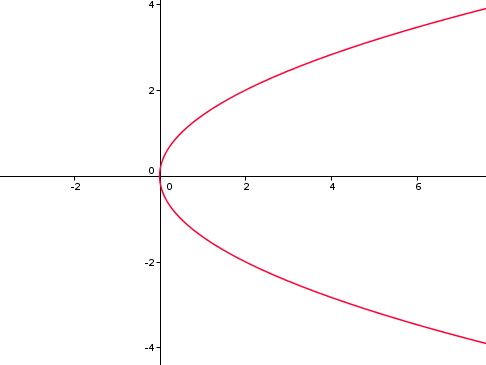
\includegraphics[scale=0.35]{img/parabola2.png}
	\end{center}
	
	Fibra sobre $\{a\}\in\{\A_k^1 \}$ puede ser varias cosas: $\varphi^{-1}(\{a\})$ puede ser 2 puntos, 1 punto o el vacío
\end{example}

Nuestro objetivo es usar el ideal de definición de W ($\I(W) \subset \K[y_1,...,y_m]$) para calcular la fibra de $\varphi$ sobre $W$.

\obs Como $W \subset Y$, entonces $\I(Y) \subset \I(W)$ por lo tanto $\I(W)$ esta en correspondencia biyectiva con el ideal $\quot{\I(W)}{\I(Y)}$ de $\K[Y]=\quot{\K[y_1,...,y_m]}{\I(Y)}$.

\subsection{Descripción algebraica de la fibra de $\varphi$ sobre $W \subset Y$:}

\begin{align*}
	\varphi: X & \rightarrow Y \\
	(a_1,...,a_n) &  \rightarrow (f_1(a_1,...,a_n),...,f_m(a_1,...,a_n))
\end{align*}

$f_i$ regulares en X.
Y. Por otro lado tenemos el homomorfismo inducido siguiente:

\begin{align*}
\varphi^*: \K[Y] & \rightarrow \K[X] \\
\cls{y_i} & \rightarrow f_i\\
\cls{G(y_1,...,y_n)} & \rightarrow \cls{G(f_1,...,f_m)}
\end{align*}

Sea $(a_1,...,a_n) \in X$ ¿Cuando $\varphi(a_1,...,a_n) \in W$?:

$\varphi(a_1,...,a_n) \in W \Leftrightarrow (f_1(a_1,...,a_n),...,f_m(a_1,...,a_n)) \in W \Leftrightarrow \forall F(y_1,...,y_m) \in \I(W)$ se tiene que $F((f_1(a_1,...,a_n),...,f_m(a_1,...,a_n))=0 \Leftrightarrow \forall F \in \I(W), \psi(F)(a_1,...,a_n)=0$.

\textbf{Conclusión:}

$$ \varphi^{-1}(W)=\left\{ (a_1,...,a_n) \in X \subset \Akn: \forall F \in \I(W), \psi(F)(a_1,...,a_n)=0 \right\} $$

En este diagrama:


\begin{tikzcd}
	\K[Y]=\quot{\K[y_1,...,y_m]}{\I(Y)} \arrow[rightarrow]{rr}{\varphi^*}
	\arrow[leftarrow]{dr}{\pi}
	& & \K[X]=\quot{\K[x_1,...,x_n]}{\I(X)}
	\arrow[leftarrow]{dl}{\psi}\\
	& \K[y_1,...,y_m]&
\end{tikzcd}

En realidad lo que hago es coger $\I(W) \in \K[y_1,..,y_m]$ o $\quot{\I(W)}{\I(Y)} \in \K[Y]$ que es lo mismo. Y los llevo a $\psi(\I(W)) \in \K[X]$.

De aquí deducimos que $\varphi^{-1}(W)=\V(\psi(\I(W))) \subset \Akn$

\begin{example}
	\begin{align*}
	\varphi: \A^2_K & \rightarrow \A^1_K \\
	(a,b) & \rightarrow a
	\end{align*}
	
	Con $|K|=\infty$
	
	Fijamos $W=\{a\} \subset \A_K^1$ y queremos calcular $\psi^{-1}(W)$.
	
	Miramos el homomorfismo de anillos que induce:
	
	\begin{align*}
	\varphi^*: \K[y_1] & \rightarrow \K[x_1,sx2] \\
	y_1 & \rightarrow x_1
	\end{align*}
	
	Vemos que $\varphi^*$ es inyectivo. Por tanto por lo que hemos visto otros días $\varphi$ debería ser dominante, y de hecho lo es, ya que es sobreyectivo. Ahora vamos a lo nuevo, a calcular la fibra sobre $\{a\}$.
	
	Para ello calculo $\I(W)$, y tenemos claramente que $\I(\{a\})=\gen{y_1 -a}$.
	
	Además $\varphi^*(\gen{y_1-a})=\gen{x_1-a}^e$. (Recordemos lo de elevar a e, que no es más que el extendido. Esto sale de que de normal en un homomorfismo la imagen $J$ de un ideal $I$ no tiene por que ser un ideal, al poner $J^e$ nos referimos al ideal más pequeño que contiene a J)
	
	Entonces $\varphi^{-1}(W)= \V(\gen{x_1-a}) \subseteq \A^2_K$. Que es una recta como vimos anteriormente.
\end{example}


\begin{example}
	\begin{align*}
	\varphi: P=\{ x_1-x_2^2=0 \} & \rightarrow \A^1_K \\
	(a,b) & \rightarrow a 
	\end{align*}
	
	Con $|K|=\infty$
	
	\begin{align*}
	\varphi: \K[y_1] & \rightarrow \quot{\K[x_1,X_2]}{\gen{x_1-x_2^2}} \\
	y_1 & \rightarrow \cls{x_1}
	\end{align*}
	
	Sea $W=\{a\} \subset \A^K_1$, entonces $\I(W) = \gen{y_1-a}$, calculo $(\varphi^*(\I(W)))^e=\gen{x_1-a} \subset \quot{\K[x_1,x_2]}{\gen{x_1-x_2^2}}$. Pero ahora CUIDADO, ese ideal no es lo mismo que $\gen{x_1-a} \subset \K[x_1,x_2]$, este último es una recta como en el ejemplo anterior.
	
	Pero los ideales de $\quot{\K[x_1,x_2]}{\gen{x_1-x_2^2}}$ están en correspondencia biyectiva con los ideales de $\K[x_1,x_w]$ que contengan a $\gen{x_1-x_2^2}$.
	
	De modo que $\gen{x_1-a} \in \quot{\K[x_1,x_2]}{\gen{x_1-x_2^2}} $ y $ \gen{x_1-a,x_1-x_2^2} \in \K[x_1,x_2]$ están en correspondencia biyectiva y es el que tengo que tomar. Ahora resuelvo el sistema para ver cuál es la v.a.a.: (consideramos $\K=\real$)
	
	$$ 
	\left\{ \begin{array}{c}
	x_1=a \\
	x_1-x_2^2=0\\
	\end{array} \right.
	\implies 
	\left\{ \begin{array}{c}
	\text{Si } a=0 \implies x_1=0, x_2=0 \\
	\text{Si } a >0 \implies x_1=a, x_2=\pm \sqrt{a}\\
	\text{Si } a < 0 \implies x_1=a, x_2^2<0 \implies \emptyset.\\
	\end{array} \right.
	$$
	
	
\end{example}

\obs: En la proyección del primer ejemplo la extension $\K[y_1]$ sobre $\K[x_1,x_2]$ no es finita porque $x_2$ no es entero sobre $\K[y_1]$

Pero en el segundo ejemplo si, ya que hemos añadido $\cls{x_2}$ que es entero  sobre $\K[y_1]$ y por tanto la extensión es finita.

